\documentclass{article}
\author{David A. Knowles}
\date{September 2015}

%\usepackage[utf8]{inputenc}
\usepackage{fullpage}%, palatino}
\usepackage{graphicx}
%\usepackage{palatino}
\usepackage{setspace}
\usepackage{helvet}
\usepackage[hidelinks]{hyperref}
\usepackage{amsmath,amssymb}
\doublespacing
\usepackage{color,soul}
%\usepackage{natbib}
\usepackage{titlesec}
\bibliographystyle{naturemag_noURL}
%\bibliographystyle{naturemag}
\usepackage[super]{natbib}
\setcitestyle{citesep={,}}
\titleformat*{\section}{\large\bfseries}
\titleformat*{\subsection}{\normalsize\bfseries}

\date{}

\begin{document}

{\Large Determining the genetic basis of anthracycline-cardiotoxicity by molecular response QTL mapping in induced cardiomyocytes}\newline

\vspace{1cm}

\noindent{\normalsize David A Knowles$^{1,2,3,*}$, Courtney Burrows$^{4,*}$, John Blischak$^{4}$, Kristen M. Patterson$^{4}$, Carole Ober$^{4}$, Jonathan K Pritchard$^{1,5,6}$, Yoav Gilad$^{4,7}$\\
\footnotesize{$^{1}$ Department of Genetics, Stanford University, Stanford, CA}\\
\footnotesize{$^{2}$ Department of Computer Science, Stanford University, Stanford, CA}\\
\footnotesize{$^{3}$ Department of Radiology, Stanford University, Stanford, CA}\\
\footnotesize{$^{4}$ Department of Human Genetics, University of Chicago, Chicago, IL}\\
\footnotesize{$^{5}$ Department of Biology, Stanford University, Stanford, CA}\\
\footnotesize{$^{6}$ Howard Hughes Medical Institute, Stanford University, CA.}\\
\footnotesize{$^{7}$ Department of Medicine, University of Chicago, Chicago, IL}\\
\footnotesize{* These authors contributed equally to this work.}\\

\section*{Introduction}

Anthracyclines, including the prototypical doxorubicin, continue to be used as chemotherapeutic agents treating a wide range of cancers, particularly leukemia, lymphoma, multiple myeloma, breast cancer, and sarcoma. 
A well-known side-effect of doxorubicin treatment is anthracycline-induced cardiotoxicity (ACT). 
For some patients ACT manifests as an asymptomatic reduction in cardiac function, as measured by left ventricular ejection fraction (LVEF), but in more extreme cases ACT can lead to congestive heart failure (CHF). 
The risk of CHF is dosage-dependent: the earliest study estimated 3\% of patients at 400 mg/m2, 7\% of patients at 550 mg/m2, and 18\% of patients at 700 mg/m2 develop CHF\cite{Swain2003}, where a more recent study puts these numbers at 5\%, 26\% and 48\% respectively. 
Reduced LVEF shows a similar dosage-dependent pattern, but is not fully predictive of CHF. 
%ACT prevalence rates in pediatric patients are notably higher \cite{todo}. 
Perhaps most daunting for patients is that CHF can occur years after treatment: out of 1,807 cancer survivors followed for 7 years in a recent survey a third died of heart diseases compared to 51\% of cancer recurrence \cite{vejpongsa2014prevention}. 




Various candidate gene studies have attempted to find genetic determinants of ACT, but are plagued by small sample sizes and unclear endpoint definitions, resulting in limited replication between studies. 
Two ACT genome-wide association studies (GWAS) have been published. 
While neither found genome-wide significant associations using their discovery cohorts, both found one variant that they were able to replicate in independent cohorts. 

A nonsynonymous coding variant, rs2229774, in RARG (retinoic acid receptor $\gamma$) was associated with pediatric ACT using a Canadian European discovery cohort of 280 patients\cite{Aminkeng2015}, and replicated in both a European ($p=0.004$) and non-European cohort ($p=1 \times 10^{-4}$). 
RARG negative cell lines have reduced retinoic acid response element (RAREs) activity and reduced suppression of \emph{Top2b}\cite{Aminkeng2015}, which has been proposed as a mediator of ACT. 

% 794 + 51
A GWAS in 845 patients with European-ancestry from a large adjuvant breast cancer clinical trial, 51 of whom developed CHF, found no variants at genome-wide significance levels\cite{Schneider2016} , but rs28714259 ($p=9 \times 10^{-6}$ in discovery cohort) replicated in two further cohorts ($p=0.04, 0.018$). 
rs28714259 falls in a glucocorticoid receptor protein binding peak, which may play a role in cardiac development. 

An exciting approach to studying human disease is to use induced pluripotent stem cell (iPSC)-derived cells as model systems for disease. Work by us and others has demonstrated that iPSCs and iPSC-derived cell-types are powerful model systems for understanding cell-type specific genetic regulation of transcription \citep{Thomas2015,Burrows2016,Banovich091660,Kilpinen2017}, but it is less established whether these systems can be used to model the interplay of genetic and environmental factors in disease progression. Encouragingly, the response of iPSC-derived cardiomyocytes (ICs) to doxorubicin was recently extensively characterized\cite{Burridge2016}. ICs derived from four individuals who developed ACT after doxorubicin treatment (``DOXTOX'' group) and four who did not (``DOX'' group), showed clear differences in viability (via apoptosis), metabolism, DNA damage, oxidative stress and mitochondrial function when exposed to doxorubicin, suggesting that ICs recapitulate \emph{in vivo} differences in doxorubicin sensitivity. Gene expression response differences between the DOX and DOXTOX groups were demonstrated using RNA-sequencing, but the sample size was insufficient (3 DOX vs. 3 DOXTOX) to attempt mapping of genetic variants that might explain the observed functional differences between lines. 

Here we use a panel of iPSC-derived cardiomyocytes from 45 individuals, exposed to four different drug concentrations, to map the genetic basis of doxorubicin-sensitivity. We find hundreds of genetics variants that modulate the  transcriptomic response, including 46 that act on alternative splicing. We show that the IC transcriptomic response is predictive of cardiac troponin response in these cell-lines, and that troponin response is itself predictive of ACT. Finally we demonstrated that the mapped genetic variants show significant enrichment in lower ACT GWAS $p$-values. 

\section*{Results}

\begin{figure}
\begin{center}
    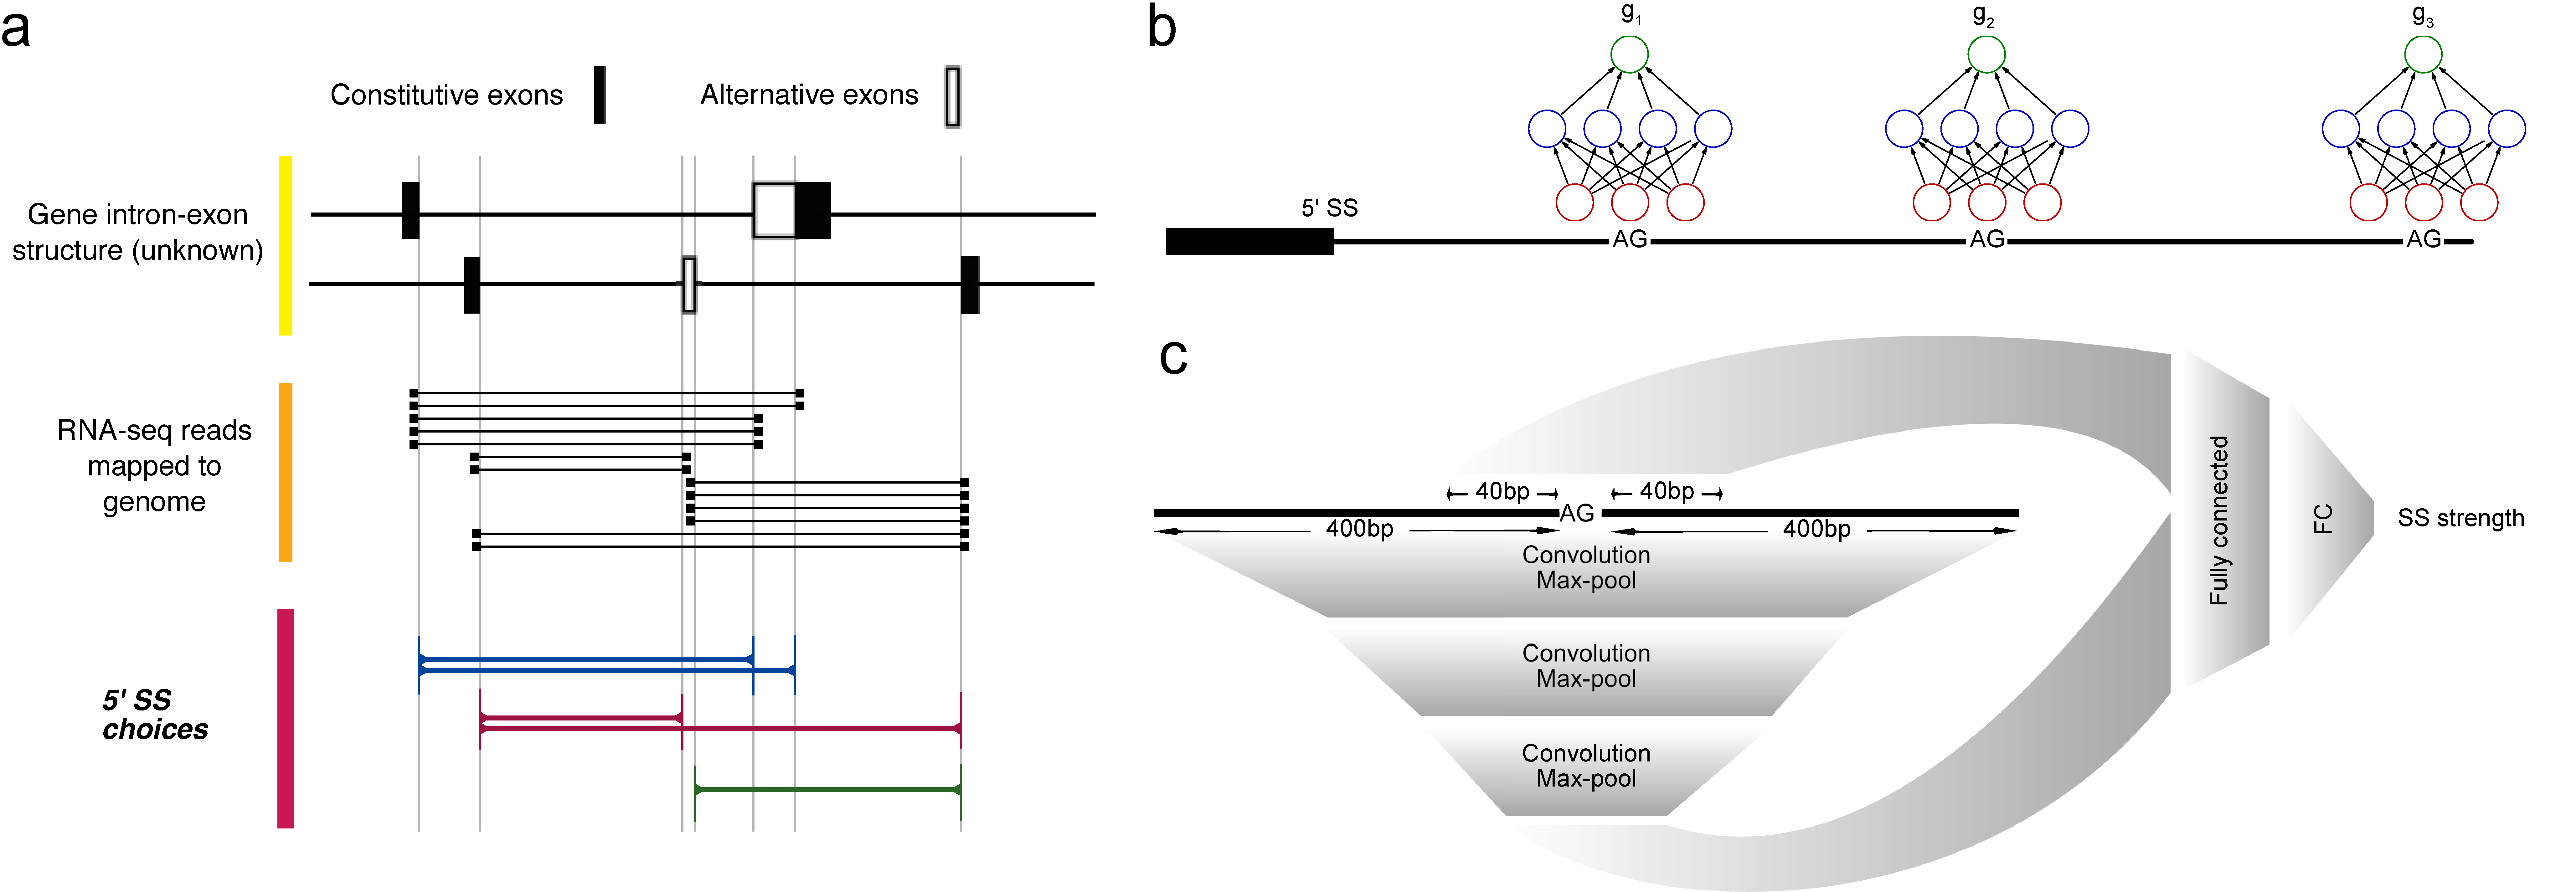
\includegraphics[width=1\textwidth]{../figures/fig1.pdf} 
        \caption{\it{The transcriptomic response of cardiomyocytes to doxorubicin is substantial. \textbf{a.} Cardiomyocytes were derived from lymphoblastoid cell lines (LCLs) of 45 Hutterite individuals, followed by exposure to differing concentrations of doxorubicin and RNA-sequencing. \textbf{b.} PCA of gene expression levels across samples reveals that doxorubicin concentration explains more variance than inter-individual differences, and that the response is non-linear with respect to concentration. \textbf{c.} A probabilistic mixture model uncovers six distinct patters of response across genes.}}
    \label{fig1}
    \end{center}
\end{figure}

\subsection*{Measuring transcriptomic response to doxorubicin exposure}

We successfully generated iPSC-derived cardiomyocytes (ICs) for 45 Hutterite individuals (Figure 1a), and confirmed cardiomyocyte identity (see Methods). We exposed all 45 IC lines to doxorubicin at 5 different concentrations for 24 hours, after which cells were processed for RNA-sequencing. We obtained sufficient read depth (10M exonic reads) for downstream analysis for 217 of the $5 \times 45 = 225$ individual-concentration pairs, and confirmed sample identity by calling exonic SNPs. We observed a strong response to doxorubicin across all concentrations, with 98\% (12038 / 12317) of quantifiable genes (5\% FDR) showing differential expression across concentrations. Our data shows excellent concordance with an existing smaller RNA-seq dataset\cite{Burridge2016} (Supplementary Figure \ref{fig:burridge}). Principal component analysis (PCA, Figure 1b) confirms that the main variation in the data is driven by doxorubicin concentration and that the effect of concentration on expression is nonlinear. For some individuals the $1.25\mu M$ sample is closer to $0.625 \mu M$, whereas for others it is closer to $2.5\mu M$, suggesting there is systematic variation in how different individuals respond to doxorubicin exposure. Since the majority of genes appear responsive to doxorubicin we clustered genes into six distinct response patterns using a mixture model approach (Figure 1c, see Methods). From largest to smallest, these clusters represent genes that are 1) down regulated 2) initial up, then further down-regulated 3) up-regulated 4) transiently down regulated 5) transiently up-regulated 6) down-regulated then partially recover. Gene set enrichments (Supplementary Figure~\ref{fig:go}) for the up-regulated cluster include metabolic, mitochrondrial and extracellular processes, as well as known doxorubicin response genes in breast cancer cell lines \cite{graessmann2007chemotherapy}. The down-regulated cluster shares genes with those down-regulated in response to UV light, which, like doxorubicin, causes DNA-damage. Targets of p53, a transcription factor that responds to DNA damage, are overrepresented in clusters 2 and 5; these clusters involve up-regulation at low concentrations ($0.625\mu M$) but down-regulation at higher concentrations. Promoter analysis (Supplementary Figure~\ref{fig:tf}) revealed 21, 45, and 6 significantly enriched transcription factor (TF) binding motifs for clusters 1, 2 and 3 respectively (and none for cluster 4-6). Examples include ZNF145, a TF that promotes GPX1 activity and protects cells from oxidative damage during mitochondrial respiratory dysfunction\cite{Lu2012}, which is enriched in cluster 1 (down regulation w/ dox); Ronin, a regulator of mitochrondrial development and function\cite{Poche2016}, which is enriched in clusters 1 and 2; and Mef2, myocyte enhancer factor 2, involved in regulating muscle development, stress-response and p38-mediated apoptosis\cite{Zarubin2005}, enriched in cluster 4 (although only at $q=0.33$).

\subsection*{Mapping variants modulating doxorubicin response}

\begin{figure}
\begin{center}
    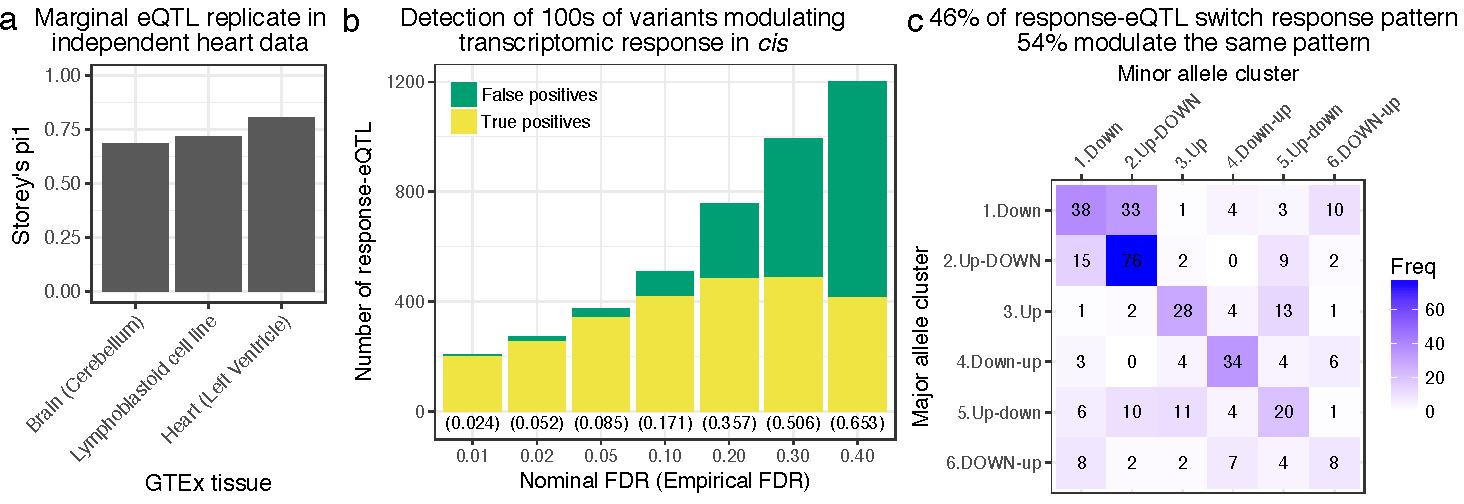
\includegraphics[width=1\textwidth]{../figures/fig2.pdf}     \caption{\it{Genetic variation regulates the transcriptomic response to doxorubicin exposure. \textbf{a.} Marginal eQTLs show strong replication in GTEx heart data, and lower replication in other tissues. \textbf{b.} We detect 100s of response-eQTLs (reQTLs): variants that modulate response to doxorubicin. The false positive rate (FPR) is estimated using a parametric bootstrap. \textbf{c.} We developed a statistical method to assign the major and minor allele response to one of the six clusters from Figure 1c. The strongest 46\% of detected reQTLs result in a discretely different response, whereas the remainder only modulate the response. \textbf{d.} We calculated relative genotype effect sizes by dividing the fitted effect size at each concentration by the (signed) effect size with the largest absolute value. $K$-means clustering of these effect size profiles reveals distinct patterns, the most common being a small reduction in absolute effect size from $0$ to $0.625\mu M$ followed by the largest effects being at the highest concentrations. \textbf{e.} An example response-eQTL where rs112594884 regulates the response of the mitochondrial complex I chaperone NDUFAF1. Under the major (T) allele we see moderate down-regulation at $0.625\mu M$ followed by up-regulation at higher concentrations. Under the minor (G) allele, there is little change at $0.625\mu M$ followed by substantial down-regulation. Since the genotype effects are reduced at $0.625\mu M$ and largest at high concentrations this reQTL is assigned to cluster 1 of panel \textbf{d}.}}
    \label{fig2}
    \end{center}
\end{figure}

We next sought to map single nucleotide polymorphisms (SNPs) that modulate the observed transcriptomic response to doxorubicin, leveraging genetic variation across the 45 individuals. We developed a linear mixed model approach, called \texttt{suez} that extends the PANAMA framework\citep{Fusi2012} to account for relatedness amongst individuals, repeat measurements, multiple conditions and latent confounding. Testing SNPs within 1Mb of the transcription start site (TSS), 518 genes have a variant with a detectable marginal effect on expression (5\% FDR). Reassuring, these eQTLs replicate in GTEx heart tissue, and do so more strongly than in GTEx brain or lymphoblastoid cell line (LCL) data (Figure 2a). Remarkably, even with our moderate number of individuals, we are able to detect many response-eQTLs (reQTLs), i.e. variants that modulate transcriptomic response to doxorubicin. We find reQTLs for 376 genes at a nominal 5\% FDR, which we estimate using a parametric bootstrap corresponds to a true FDR of $8.5\%$ (Figure 2b). 

To characterize the detected reQTLs we assigned the response of the major and minor allele to one of the six clusters previously learned (Figure 1c), with heterozygotes expected to display the average of the two homozygous responses. 172 (46\%) of reQTLs result in a qualitatively distinct response as determined by the two alleles being assigned to different clusters. The most common transition, occurring for 33 reQTLs, is that the major allele is associated with simple down-regulation (cluster 1) in response to doxorubicin, whereas the minor allele shows a transient up-regulation at low concentration followed by down-regulation at higher concentration (cluster 2). 

We further broke-down the significant reQTLs by considering the effect of genotype on expression at each concentration ($\beta_c$ in Equation~\ref{eq:betac}). We normalized relative to the $\beta_c$ with the largest absolute value, i.e. we consider $\beta_c / \beta_{\arg \max{ |\beta_{c'}| }} $, so that the largest genotype effect always corresponds to a normalized value of 1. The resulting normalized effect profiles were split into 9 clusters using $k$-means clustering (Figure 2d). The largest cluster (cluster 1, 85 reQTLs) represents reQTLs with a modest effect size at low concentrations ($0,0.625\mu M$) which is amplified at higher concentrations (Figure 2e shows a highly significant example). Cluster 2 corresponds to reQTLs whose effect size is attenuated at $0.625\mu M$: examples in this cluster tend to have higher expression that $0.625\mu M$ and what could be buffering of very high expression levels which reduces the genetic effect (e.g. rs16853200's association with ABCA12 response, Supplementary Figure \ref{fig:ABCA12}).

\subsection*{Doxorubicin exposure reduces splicing fidelity}

% Splicing and ox stress:
% https://www.ncbi.nlm.nih.gov/pubmed/18059557
% http://journals.plos.org/plosone/article?id=10.1371/journal.pone.0154390
% http://gut.bmj.com/content/61/Suppl_2/A123.2
% https://www.ncbi.nlm.nih.gov/pubmed/27591253

Oxidative stress, a major downstream consequence of doxorubicin exposure, disrupts splicing of individual genes including HPRT and POLB\cite{Disher2007}, and SMA\cite{Seo2016}. We queried the extent to which doxorubicin exposure disrupts splicing patterns across the transcriptome using \texttt{LeafCutter}\cite{LeafCutter}. Across all samples \texttt{LeafCutter} detected 27769 alternative splicing ``clusters'' (referred to here as ``ASCs'' to avoid confusion with $k$-means clusters) , which correspond approximately to splicing events, with a median of 3.0 splice junctions per ASC. 10430 (59\%) ASCs, corresponding to 6398 unique genes, showed an effect of doxorubicin exposure on splicing outcomes (5\% FDR). To characterize these changes we calculated the entropy of the splicing choices made for each significant ASC at each concentration and used $k$-means clusters patterns of change in entropy (Figure \ref{fig_splicing}a). The largest cluster has 6166 ASCs (59\%), and corresponds to the null of no clear change in entropy across concentrations. Clusters 2 ($n=1136$) and 5 ($n=475$) correspond to increasing entropy with concentration, and clusters 3, 4, 6, 8 and 9 correspond to the maximum entropy being at different concentrations and reaching different maximum levels. Interestingly, only the relatively small cluster 8 ($n=304, 3\%$ of ACSs) corresponds to a reduction in entropy at higher  concentrations, suggesting the dominant behavior is reduced splicing fidelity and increased alternative splicing in response to doxorubicin. 

We further tested the hypothesis that splicing fidelity decreases in the presence of doxorubicin by comparing patterns of intronic $\Psi$ with canonical vs cryptic (unannotated) splice site usage. We clustered the 7792 introns in significantly differentially spliced ASC, that have $\Delta \Psi > 0.1$ for some pair of concentrations, into 8 response patterns based on their relative excision proportions across concentrations. For each cluster we calculated the proportion of member introns with neither end annotated, one end unannotated, or both ends annotated (Figure \ref{fig_splicing}b). The clusters representing increased $\Psi$ with concentration (clusters 2, 4, 6 and 7) all show enrichment for cryptic splice site usage. The two most populous clusters (1 and 2) correspond to $\Psi$ decreasing and increasingly continuously with doxorubicin concentration, respectively, and the difference in levels of cryptic splicing is extremely apparent (hypergeometric $p < 2 \times 10^{-16}$, odds ratio for one annotated end vs two is $28.0$).

\begin{figure}
\begin{center}
    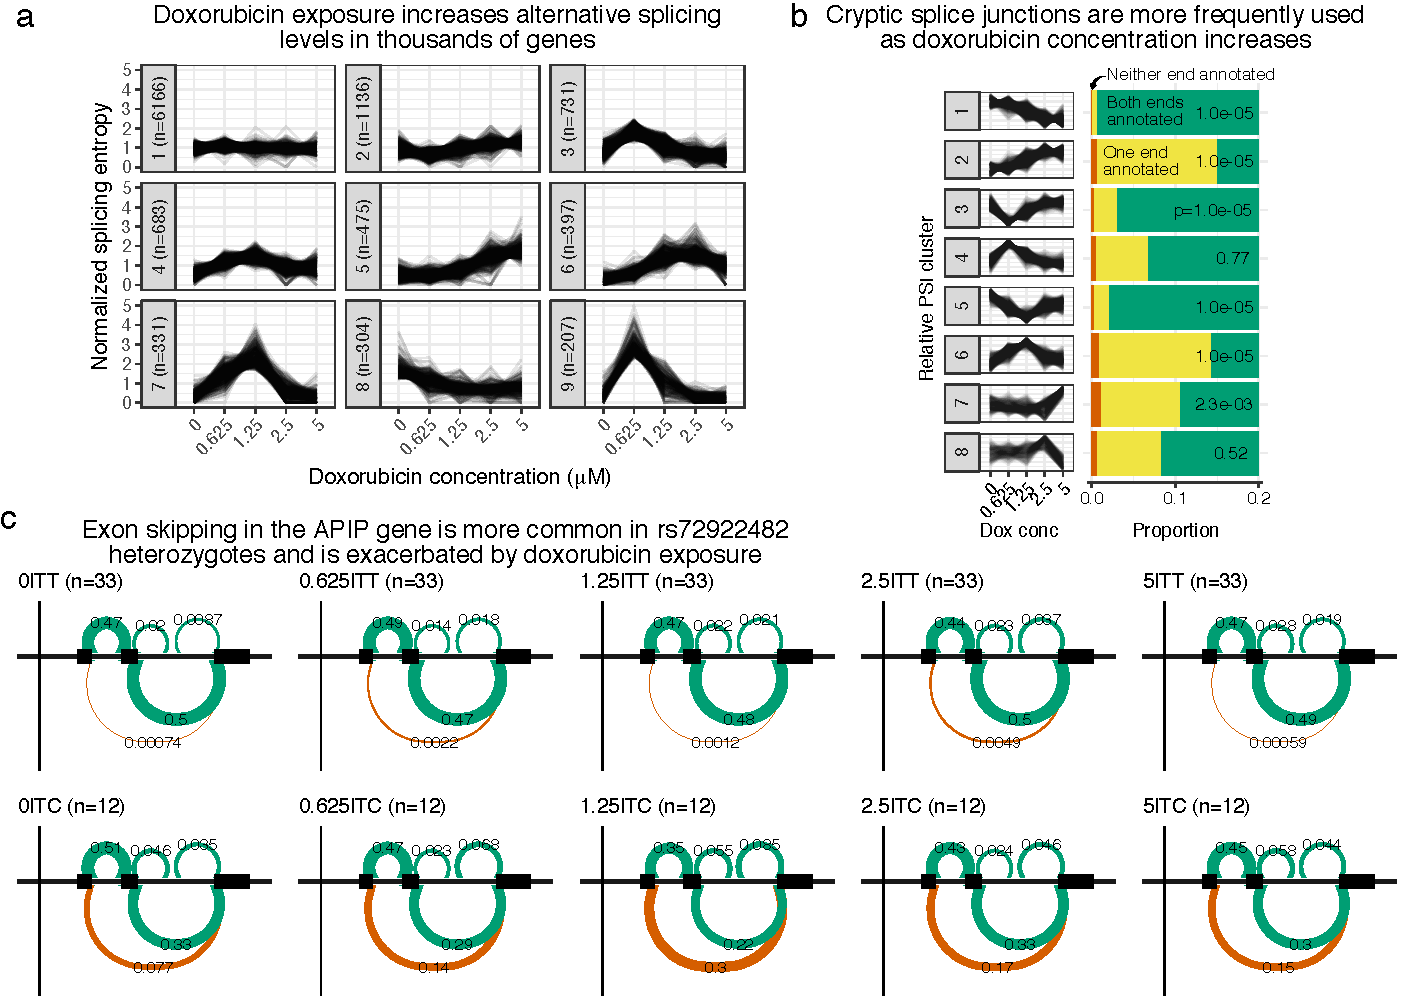
\includegraphics[width=1\textwidth]{../figures/fig3_splicing.pdf}     \caption{\it{Doxorubicin exposure significantly impacts alternative splicing. \textbf{a} The entropy of splicing choices increases in response to doxorubicin exposure. We measured splicing entropy at different concentrations within \texttt{LeafCutter} ``Alternative Splicing Clusters'' (ACSs) and clustered these into patterns of entropy change. \textbf{b} We separated introns differentially excised with $\Delta \Psi > 0.1$ into 8 clusters based on their relatively excision level at each concentration. Introns in clusters corresponding to increased excision at higher doxorubicin concentrations (e.g. cluster 2) are far more likely to use a cryptic (unannotated) splice site at at least one end. $p$-values shown are for a hypergeometric test of that cluster against all others. \textbf{c} We mapped 42 ASCs with response splicing QTLs, variants that modulate the differential splicing response to doxorubicin.}}
    \label{fig_splicing}
    \end{center}
\end{figure}

We additionally used \texttt{LeafCutter} quantification of percentage spliced in (PSI) for each splice junction to map splicing QTLs (sQTL) and response-splicing QTLs (rsQTL) using the same methodology as we employed for reQTL mapping. We tested SNPs within 100kb of either end of the splice junction. At 5\% FDR we found 467 ASCs with a marginal effect sQTL and 42 with a rsQTL. An example rsQTL is rs72922482's association with inclusion of exon 2 of APAF1 Interacting Protein (APIP). Under the major T allele exon skipping is extremely rare: the \texttt{LeafCutter} PSI for the spanning junction ranges from $0.00059$ to $0.0049$ across concentrations (Figure \ref{fig_splicing}c). In rs72922482 heterozygotes however the exon is skipped in a significant proportion of transcripts, and this effect is most pronounced at $1.25 \mu M$, with approximately 50\% exon inclusion, suggesting the minor C allele results in very low inclusion of the cassette exon. Another interesting example is NDUFAF6, another mitochrondrial Complex I protein, where doxorubicin exposure (particularly at $0.625 \mu M$) results in increased use of an alternative downstream transcription start site (TSS) which unmasks the influence of rs896853 on a cassette exon between the two alternative TSS (Supplementary Figure \ref{fig:NDUFAF6}).

\subsection*{Transcriptional response to doxorubicin is predictive of the cardiac-damage indicator troponin}


\begin{figure}
\begin{center}
    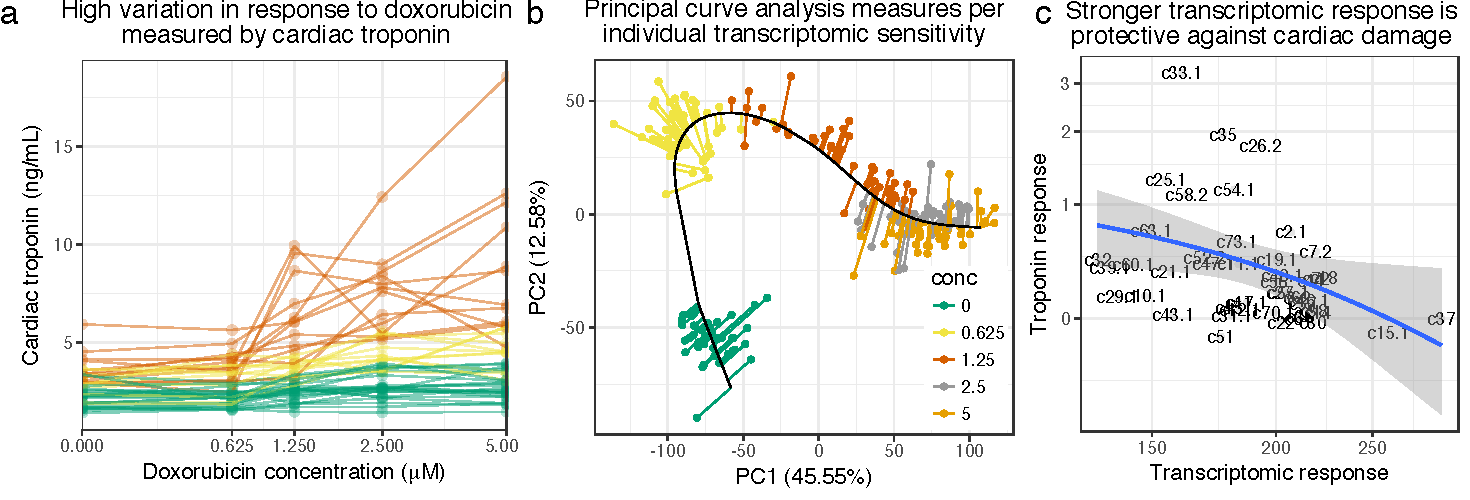
\includegraphics[width=1\textwidth]{../figures/fig4_troponin.pdf}     \caption{\it{Transcriptomic response is predictive of doxorubicin induced damage as measured by cardiac troponin. \textbf{a.} We measured cardiac troponin, a sensitive and specific test for myocardial damage, in response to doxorubicin, across all cell lines. \textbf{b.} We performed differential expression analyses with respect to troponin at each concentration separately, and observed more differentially expressed genes at higher concentrations corresponding to an increased dynamic range of troponin response. \textbf{c.} We took differentially expressed genes (5\% FDR) at each concentration and checked for ``replication'' $($nominal $p<0.05)$ at the other concentrations. Note that no differentially expressed genes were discovered in control condition $(0 \mu M)$. \textbf{d.} We summarized gene expression response by first fitting a ``principal curve'' following increasing doxorubicin concentration, and then measuring the rate of progression along this curve for each individual. \textbf{e.} Increased transcriptomic response is associated with reduced cardiac troponin response, suggesting that the bulk of expression changes we observe are in fact protective against cardiac damage. \textbf{f.} Based on the observed transcriptomic response to doxorubicin in our cell lines we predicted ACT using available 3 v. 3 case/control data\cite{Burridge2016}. The probability of ACT correlated significantly with the slope of troponin response (Spearman $\rho=0.38, p=0.01$), supporting the \emph{in vivo} disease relevance of our IC system. }}
    \label{fig_troponin}
    \end{center}
\end{figure}

We used cardiac troponin to measure damage occurring as a result of doxorubicin exposure, using the same concentrations as for our expression profiling. We observed significant variation in measurable damage caused by doxorubicin across individuals, with 13 out of 45 cell lines having a significant (positive) response (Figure \ref{fig_troponin}a). We first sought to determine whether the inter-individual variation in troponin response could be explained by variation in expression response. Since we are interested in inter-individual rather than between concentration differences we normalized the troponin response to have 0 mean and variance of 1 across samples at each doxorubicin concentration. We found 96.1\% (95\% credible interval $[91.5\% 98.6\%]$) or 92.1\% of the variance in this normalized troponin response could be explained using gene expression levels at the corresponding doxorubicin concentrations, using a GREML-analysis\cite{Yang2010-cx} or leave-out-one cross validated LASSO\cite{tibshirani1996regression} respectively. The optimal LASSO model included 118 genes, listed in Supplementary Table S1. 

To further explore the relationship between transcriptomic and troponin response we analyzed differential expression (DE) with respect to troponin response at each doxorubicin concentration separately. We found 0, 7, 78, 2984 and 2863 differentially expressed genes (5\% FDR) at the 5 concentrations respectively (Figure \ref{fig_troponin}b). The most strongly DE gene at $5 \mu M$ is DUSP13, a known regulator of ASK1-mediated apoptosis\cite{park2010positive}. The large number of DE genes at $2.5 \mu M$ and $5.0 \mu M$ are broadly shared (nominal replication rate 82\% to 85\%), and DE genes at $1.25 \mu M$ generally represent the most strongly DE genes at the higher concentrations (Figure \ref{fig_troponin}c). 

To compare troponin sensitivity to transcriptomic response we determined an overall per-individual measurement of transcriptomic response with respect to doxorubicin concentration. To this end we fit a principal curve\citep{hastie1989principal} through all gene expression samples, initializing the curve to pass sequentially through the successive doxorubicin concentrations (Figure \ref{fig_troponin}d). Projecting every sample on the principal curve gives a single measure of ``progression'' through doxorubicin response. We then regressed these values against concentration for each individual to obtain a progression rate. We found the troponin response slope is significantly negatively correlated (Spearman $\rho=-0.42, p=0.004$, Figure \ref{fig_troponin}e) with the transcriptomic response rate, suggesting that much of the gene expression program being activated in response to doxorubicin is in fact protective against cardiac damage. 

We built a predictive model of ACT trained on RNA-seq of ICs exposed to $1 \mu M$ doxorubicin from patients with ($n=3$) and without ($n=3$) ACT\cite{Burridge2016} using LASSO (with fixed $\lambda=10^{-5}$). We applied this model to our expression data at $0.625 \mu M$ (since this concentration shows excellent concordance with the $1 \mu M$ data of Burridge et al., see Supplementary Figure \ref{fig:burridge}) to obtain predicted log-odds of ACT. While these log-odds are unlikely to be well-calibrated due to differences in the training and test datasets, they may still accurately represent relative risk of ACT across our 45 individuals. Indeed, the log-odds correlated significantly with the troponin response slope (Spearman correlation $p=0.01$, Figure \ref{fig_troponin}f), suggesting our troponin response data, and by extension our expression response data, recapitulate \emph{in vivo} cellular response to doxorubicin. 

\subsection*{Cardiomyocyte molecular QTLs show enrichment in ACT GWAS} 

\begin{figure}
\begin{center}
    \includegraphics[width=1\textwidth]{../figures/fig5_gwas.pdf}     \caption{\it{Cardiomyocyte molecular QTLs are enriched in ACT GWAS. \textbf{a.} rs4058287 has a GWAS $p$-value of $9.68\times 10^{-6}$ and is a nominally significant eQTL ($p=0.0016$) for ALPK2, which is down-regulated in response to doxorubicin. \textbf{b.} SNPs that have either a marginal or response eQTL with $p<10^{-5}$ are enriched in GWAS variants with $p<0.05$ (hypergeometric test $p=3 \times 10^{-6}$). \textbf{c.} SNPs with a marginal or response splicing QTL at $p<10^{-5}$ show modest enrichment in GWAS $p<0.005$ (hypergeometric $p=0.02$).}}
    \label{fig:gwas}
    \end{center}
\end{figure}

% Statistical signal for the eQTL and GWAS co-localizes for ADCY2 at rs6893414.

To determine the disease-relevance of our molecular QTLs we obtained summary statistics for the largest ACT GWAS to date\cite{Schneider2016}. While this GWAS was not sufficiently powered to find genome-wide significant associations, 11 variants representing 9 independent loci have $p<10^{-5}$, with the most significant (rs2184559) at $p=2.8 \times 10^{-6}$. Of the 8 GWAS variants with $p<10^{-5}$ either tested in our eQTL mapping, or in high LD ($R^2 > 0.8$) with a tested SNP, 7 have a nominally significant marginal eQTL ($p<0.05$, the 8th has $p=0.07$) and four have a reQTL with $p<0.1$. rs4058287 (GWAS $p$-value $9.68\times 10^{-6}$) has a marginal effect on Alpha-Protein Kinase 2 (ALPK2, also known as ``Heart Alpha-Protein Kinase'' since it was discovered in mouse heart\cite{ryazanov1999alpha} and is expressed in few other tissues\cite{Mele2015-sc}) expression ($p=0.0016$) as well as a weak interaction effect ($p=0.06$, see Figure \ref{fig:gwas}a). Interestingly, ALPK2 has been shown to upregulate DNA repair genes and to enable caspase-3 cleavage and apoptosis in a colorectal cancer model\citep{yoshida2012alpk2}. 

We additionally assessed whether there was detectable enrichment of low GWAS $p$-values for our molecular QTLs. For total gene expression we considered SNPs with either a marginal or response eQTL with nominal $p < 10^{-5}$ (corresponding approximately to 5\% FDR) and found a significant enrichment for GWAS $p$-values under $0.05$ (one-sided hypergeometric $p=3 \times 10^{-6}$, OR=$1.2$, Figure \ref{fig:gwas}b). We observed a more modest enrichment for splicing QTLs: using the same criteria to define a set of sQTL variants we observe significant enrichment in GWAS $p$-values under $0.005$ (one-sided hypergeometric $p=0.02$, \ref{fig:gwas}c) but not under $0.05$ (one-sided hypergeometric $p=0.7$).  

\section*{Discussion}

Human iPSC-derived somatic cells provide a powerful, replenishable and reproducible tool for modeling cellular responses to external perturbation \emph{in vitro}, especially for non-blood cell-types such as cardiomyocytes which are extremely challenging to collect and even then are typically only available post-mortem. 
The strong association we observed between transcriptomic and cardiac troponin response to doxorubicin, combined with existing evidence\cite{Burridge2016}, supports the \emph{in vivo} relevance of ICs to anthracycline-induced cardiomyopathy (ACT). 
The ready availability of lymphocytes as a source material allowed us to assemble a sufficiently large IC panel to effectively query not only the transcriptomic response of cardiomyocytes to doxorubicin, but also the role of genetic variation in modulating this response, both in terms of total expression and alternative splicing. 

We observed a statistical enrichment of expression and (to a lesser extent) splicing molecular QTLs in ACT GWAS. However, with no genome-wide significant associations available, fine-mapping of causal variants remains fraught. We anticipate our findings will be increasingly valuable as larger-scale ACT GWAS become available. 

We derived ICs from healthy individuals. Mapping molecular response QTLs in ICs from patients treated with anthracyclines who do or do not develop ACT symptoms would allow stronger conclusions to be drawn about the contribution of individual genetic variants to disease etiology. 

\section*{Methods} 

\subsection*{Sample collection and genotyping}

Generation of lymphoblastoid cell lines (LCLs) and genome-wide genotyping of
many individuals from a multi-generational pedigree were performed
previously. Briefly, lymphocytes were isolated from whole blood samples using
Ficoll-Paque and immortalized using Epstein Barr Virus \cite{Cusanovich2012,
Cusanovich2016}. Phased genotypes were obtained by combining pedigree
information, genotypes from SNP arrays, and genotypes from whole genome
sequencing of related individuals \cite{Livne2015}.

\subsection*{iPSC reprogramming and cardiomyocyte differentiation} 

We reprogrammed the 45 LCLs to iPSCs using episomal plasmid vectors,
which avoids integrating additional transgenes \cite{Okita2011}. We
chacterized the iPSC lines using the embryoid body assay, karyotyping,
and the PluriTest \cite{Muller2011} classifier. Next we differentiated
the iPSCs to cardiomyocytes \cite{Lian2013, Burridge2014} and assayed
purity by performing flow cytometry for cardiac Troponin T.

\subsection*{Doxorubicin exposure}

We incubated the cardiomyocytes in 0, 0.625, 1.25, 2.5, or 5 $\mu$M
doxorubicin. After 24 hours, we collected the serum and cells from each
condition. From the serum, we measured cardiac Troponin T levels using the
ABNOVA Troponin I (Human) ELISA kit (cat. no. KA0233). From the cells, we
extracted RNA for sequencing. Each treatment batch contained 1 to 4
individuals. RNA quality was assessed with the Agilent Bioanalyzer.

\subsection*{RNA-sequencing}

We prepared libraries using the Illumina TruSeq Library Kit and
generated 50 bp single-end reads on a HiSeq 4000 at the University of
Chicago Functional Genomics Facility. The reads were 50 bp single
end. We confirmed sequencing quality using FastQC and MultiQC
\cite{Ewels2016}. We confirmed sample identity by 1) comparing
allelic counts of exonic SNPs to the known genotypes and 2) running
verifyBamID \cite{Jun2012}.

\subsection*{Expression quantification}

We aligned RNA-seq reads using STAR version 2.5.2a \cite{Dobin2013} to GRCh38/GENCODE release 24. We counted reads using featureCounts \cite{Liao2014} and calculated counts per million reads (cpm) using `cpm` from the `edgeR` R package (version 3.18.1) \cite{Robinson2010}. We discarded samples with $<10^9$ reads and genes with median $\log_2(cpm)$ less than $0$.

\subsection*{Differential expression analysis} 

We performed differential expression (DE) analysis across all 5 doxorubicin concentrations jointly, using either a linear model on quantile normalized cpm value or Spearman correlation, followed by Benjamini-Hochberg False Discovery Rate (FDR) control. Since the vast majority of genes showed differential expression we did not investigate better powered DE methods such as DESeq2. 

We clustered genes into ``response patterns'' using a $K$-component mixture model 
\begin{align}
\pi &\sim \text{Dir}(1/K,\cdots,1/K) \nonumber \\ 
z_g | \pi &\sim \text{Discrete}(\pi) \nonumber \\
y_{ngc} | z_g, \theta &\sim N( \theta_{cz_g}, \sigma^2 )
\label{eq:mixture}
\end{align}
where $\pi$ is a prior probability vector over cluster assignments, Dir is the Dirichlet distribution, $z_g$ is cluster from which gene $g$ is generated, $y_{ngc}$ is the expression of gene $g$ in individual $n$ at concentration $c$, $\theta_{ck}$ is the mixture parameter (mean) across concentrations for cluster $k$, and $\sigma^2$ is a shared noise variance. 
We marginalize (sum) over $z_g$ and optimize with respect to $\pi, \theta, \sigma$ using the RStan R package (version 2.16.2). 
The hyperparameters of the Dirichlet distribution are set such that in the limit of large $K$ the model approximates a Dirichlet process mixture \cite{maceachern1998estimating} which automatically learns of an appropriate number of mixture components to use from data. 

Gene set and promoter motif enrichment was performed using HOMER v4.9.1\cite{heinz2010simple} using default parameters and without \emph{de novo} motif search. 

\subsection*{Response eQTL mapping} 

We developed an extension of the PANAMA\cite{Fusi2012} linear mixed model (LMM) framework to map eQTLs and response eQTLs while accounting for latent confounding, which we call \texttt{suez}. \texttt{suez} entails a two step procedure. Step one is used to learn latent factors from all genes, using the model
\begin{align*}
y_{ncg} &= \sum_k W_{kg} x_{nck} + u_{ng} + v_{cg} + \xi_{ncg} + \epsilon_{ncg} \\
W_{kg} & \sim N(0, \sigma^2_k ) \qquad \textit{ factor loadings/coefficients } \\ 
u_{ng} &\sim N(0, \sigma^2_u) \qquad \textit{ individual random effects } \\
\xi &\sim MVN(0, \sigma^2_\xi \Sigma ) \qquad \textit{ kinship random effect }  \\
\epsilon &\sim MVN(0, \text{diag}(\sigma^2_\epsilon)) \qquad \textit{ noise } 
\end{align*}
where $x_{nck}$ are latent factors, $v_{cg}$ are per gene, per concentration fixed effects. We integrate over $W, u, \xi$ and $\epsilon$, which results in a per gene multivariate normal,
\begin{align}
y_{:g} \sim MVN\left( V v_{:g} , \sum_k \sigma^2_k x_{:k} x_{k:}^T + \sigma^2_u U + \sigma^2_\xi \Sigma + \sigma^2_e I \right),
\end{align}
where $y_{:g}$ refers to the vector of expression for gene $g$ across all individuals and concentrations (i.e. all ``samples'' where a sample is an individual-concentration pair), $V$ is a matrix mapping concentrations to samples (i.e. $V_{sc}=1$ iff sample $s$ is at concentration $c$) and $U$ is a matrix of which samples are for the same individual (i.e. $U_{ss'}=1$ if sample $s$ and sample $s'$ come from the same individual). We optimize $x,v$ and the variances $\{ \sigma^2_u, \sigma^2_k,  \sigma^2_\xi, \sigma^2_\epsilon \}$ jointly across all genes $g$. 

In step 2 we test individual gene-SNP pairs while accounting for confounding using the covariance matrix 
\begin{align}
 \Sigma_\pi = \sum_k \sigma^2_k x_{:k} x_{k:}^T + \sigma^2_u U + \sigma^2_\xi \Sigma 
 \end{align}
which includes both latent confounding, individual random effects and similarity due to kinship. We consider three LMMs, all with the same parameterization of the covariance $\sigma^2_\pi \Sigma_\pi + \sigma^2_e I$ where $\sigma^2_\pi$ and $\sigma^2_e$ are optimized along with the fixed effects to allow the extent to which each gene follows the global covariance pattern to be adapted. The simple structure of this covariance also allows pre-computation of the eigen-decomposition of $\Sigma_\pi$ which enables linear (rather than cubic) time evaluation of the likelihood and its gradient. 

Model 0 involves no effect of the SNP (and can therefore be fit once for a gene), a fixed effect for concentration. Model 1 adds a marginal effect of the SNP genotype dosage $d$. Finally model 2 adds an interaction effect between concentration and genotype, which is equivalent to a concentration-specific genotype effect. In summary: 
\begin{align}
\text{Model 0: }& \mathbb{E}[ y_{ncg} ] = v_{cg} \\ 
\text{Model 1: }& \mathbb{E}[ y_{ncg} ] = v_{cg} + \beta d_n \\
\text{Model 2: }& \mathbb{E}[ y_{ncg} ] = v_{cg} + \beta_c d_n \label{eq:betac}
\end{align}
We optimize $\sigma^2_\pi$, $\sigma^2_e$ and the regression coefficients for each of the three models separately, and use likelihood ratio tests (LRT) to compare the models. Comparing Model 1 vs 0 (one degree of freedom) tests whether there is a marginal effect of the variant. Comparing Model 2 vs 1 ($C-1=4$ degrees of freedom, where $C$ is the number of conditions/concentrations) tests whether there is an interaction effect, i.e. whether the genetic effect on expression is different at different concentrations (or equivalently whether the response to doxorubicin is different for different genotypes). Finally Model 2 vs 0 ($C=5$ degrees of freedom) tests whether there is any effect of genotype on expression, either in terms of a marginal or concentration-specific effect. We use the conservative approach of using Bonferroni correction across SNPs for a gene, followed by Benjamini-Hochberg FDR control. 

We quantile normalize the expression levels across all samples for each gene to a standard normal distribution so that the distributional assumptions of our linear mixed model are reasonable. However, optimizing the variance parameters $\sigma^2_\pi$ and $\sigma^2_e$ means that the $\chi^2$ distribution for the LRT will only hold asymptotically and $p$-values for finite sample sizes will tend to be somewhat anti-conservative. To account for this for response-eQTLs we use a parametric bootstrap since there is no fully valid permutation strategy for testing interaction effects. This involves first fitting Model 1 and then simulating new expression data under the fitted model. Models 1 and 2 are then (re)fit to this data and compared using an LRT. We then perform Bonferroni correction across SNPs for each gene to obtain an empirical null distribution of per gene $p$-values which we use to estimate the true FDR for our response-eQTL results. 

For significant reQTLs we assigned the response of the minor allele and major allele to the previously determined clusters using the model
\begin{align*}
y_{nc} | z_A,z_a, \theta &\sim N\left( \frac12 d_n \theta_{cz_A} + \frac12 (2 - d_n) \theta_{cz_a}, \sigma^2 \right),
\end{align*}
where $y_{nc}$ is the expression for individual $n$ at concentration $c$, $z_A$ and $z_a$ are the cluster assignments for the major and minor allele respectively, $d_n \in \{0,1,2\}$ is the genotype dosage, and $\theta$ and $\sigma^2$ are fixed at the values learned in Equation \ref{eq:mixture}. For each reQTL separately we calculate the likelihood of $y$ given all possible pairs of assignments $(z_A,z_a)$ and choose the maximum likelihood solution. 

As for all $k$-means clustering in the paper, we used \texttt{KMeans\_rcpp} function of the R package \texttt{ClusterR} v1.0.6, taking the best of 10 initializations using the \texttt{k-means++} option, to cluster the normalized genotype effect profiles of the significant associations. The choice of 9 clusters was determined manually. 

\subsection*{Splicing analysis}

We ran \texttt{LeafCutter} v0.2.6 using default settings and the \texttt{multiclass} github branch which allows joint differential intron excision testing across more than two conditions. For each Alternative Splicing Cluster (ASC) \texttt{LeafCutter} fits a set of $Percent Spliced In$ probability vectors $\psi_{c}$, across detected splice junctions $i$, at each concentration $c$. For ACSs determined to be significantly (5\% FDR) differential spliced across concentrations, we calculated the entropy $h_c = -\sum_i \psi_{ci} \log \psi_{ci}$ at each concentration $c$. We normalized these profiles as $\tilde{h_c} = h_c / \bar{h_c}$ and clustered these profiles, using \texttt{KMeans\_rcpp} as above. 

To investigate the relative usage of cryptic splice sites we first determined the set of 7792 splice junctions that a) fell in ASCs determined to be significantly differentially spliced (5\% FDR) and b) had $\max_c \psi_{ci} - \min_c \psi_{ci} > 0.1$. We obtained normalized intron excision rates by the per intron mean and dividing by the per intron standard deviation. These $\psi$ profiles were clustered using \texttt{KMeans\_rcpp}. Cryptic splice site usage was determined by considering all exons in Gencode v26 and ignoring transcript structure (i.e. a junction spanning two splice sites used but only in different transcripts would still be considered ``annotated''). 

For (response) splicing QTL we calculated within ASC intron excision $\psi$ with pseudocount of $0.5$, and set entries with $0$ denominator (no reads for that ASC in that sample) to the mean across all other samples. These values were then 1) $z$-score normalized across samples and 2) quantile normalized to a normal across introns. QTL mapping was then performed using \texttt{suez} considering each intron as a ``gene''. 

\subsection*{Modeling cardiac troponin response}

We assessed the proportion of variance in cardiac troponin response explained by gene expression response. Let $y_{ci}$ represent the troponin level measured in individual $i$ at doxorubicin concentration $c$, normalized to have 0 mean and variance 1 across individuals at each concentration. Let $x_{cig}$ be the expression of gene $g$ (in individual $i$ at concentration $c$), $z$-score normalized across samples. We consider the linear model 
\begin{align}
y_{ci} = \sum_g \beta_g x_{cig} + \epsilon_{ci}
\end{align}
where $\epsilon_{ci} \sim N(0,\sigma_\epsilon^2)$ is noise and the coefficients $\beta_g$ are given a prior $N(0, \sigma_\beta^2 / G )$ where $G=12,317$ is the number of genes in the analysis. Integrating over $\beta_g$ we have 
\begin{align}
y_{:} \sim N\left(0 , \sigma_\beta^2 \frac{1}{G} \sum_g x_{:g} x_{:g}^T + \sigma_\epsilon^2 I \right)
\end{align}
We optimize this model wrt $\sigma_\beta$ and $\sigma_\epsilon$ to obtain an estimate $\sigma_\beta^2 / (\sigma_\beta^2 + \sigma_\epsilon^2)$ of the percent variance of $y$ explained by $x$. 

\subsection*{Data and code availability}

The RNA-seq FASTQ files and genotype files have been deposited in and are
available from the dbGaP database \cite{Tryka2014} under dbGaP accession
phsxxxxxx.vx.px
(\url{https://www.ncbi.nlm.nih.gov/projects/gap/cgi-bin/study.cgi?study_id=phsxxxxxx.vx.px}).
The following data sets are available as Supplementary Data: 1) gene-by-sample
matrix of RNA-seq counts, 2) differential expression results, 3) classification
of genes into response patterns, 4) eQTL mapping results, 5) splicing results,
6) levels of cardiac Troponin and the predicted transriptomic response.  The
summary statistics for the ACT GWAS were given to us by the authors of the study
\cite{Schneider2016}. All the custom analysis scripts used for this project are
available at \url{https://github.com/davidaknowles/dox}.

\section*{Acknowledgement}

We gratefully acknowledge Bryan Schneider for provided GWAS summary statistics. 
TODO funding

\section*{Author Contributions}

DAK performed data analysis, algorithm development and statistics, and prepared the manuscript. 
CB performed the experiments. 
JB performed data analysis and QC. 
KMP performed sequencing. 
CO provided source material and supervision.
YG and CB conceived the project.
JKP and YG supervised the project.

\section*{[References at the end]}
\newpage

%\bibliographystyle{genres}
%\bibliography{refs}     

\setcounter{figure}{0}
\makeatletter 
\renewcommand{\thefigure}{S\@arabic\c@figure}

\section{Supplementary material} 

\begin{figure}[h]
\begin{center}
    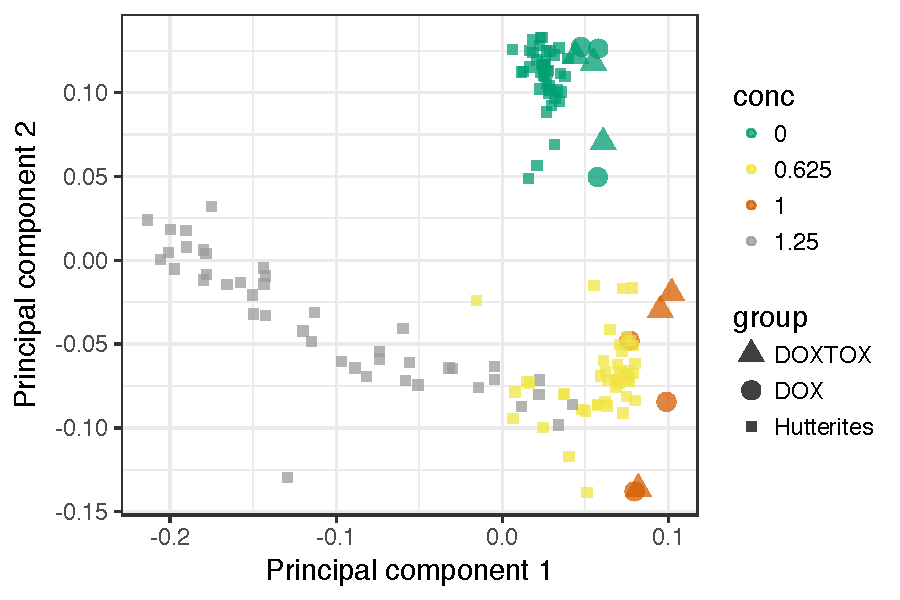
\includegraphics[width=.6\textwidth]{../figures/burridge_comparison.pdf} % use small or
    \caption{\it{Our expression data is concordant with an existing small RNA-seq dataset\citep{Burridge2016}. DOXTOX and DOX correspond to samples from patients that did and did not develop ACT after doxorubicin chemotherapy respectively. We additionally see that the transcriptional response at higher concentrations cannot be extrapolated from that at lower concentrations. Higher concentrations are not shown since including these compresses the first PC obscuring the relevant variation.}}
    \label{fig:burridge}
    \end{center}
\end{figure}

\begin{figure}[h]
\begin{center}
    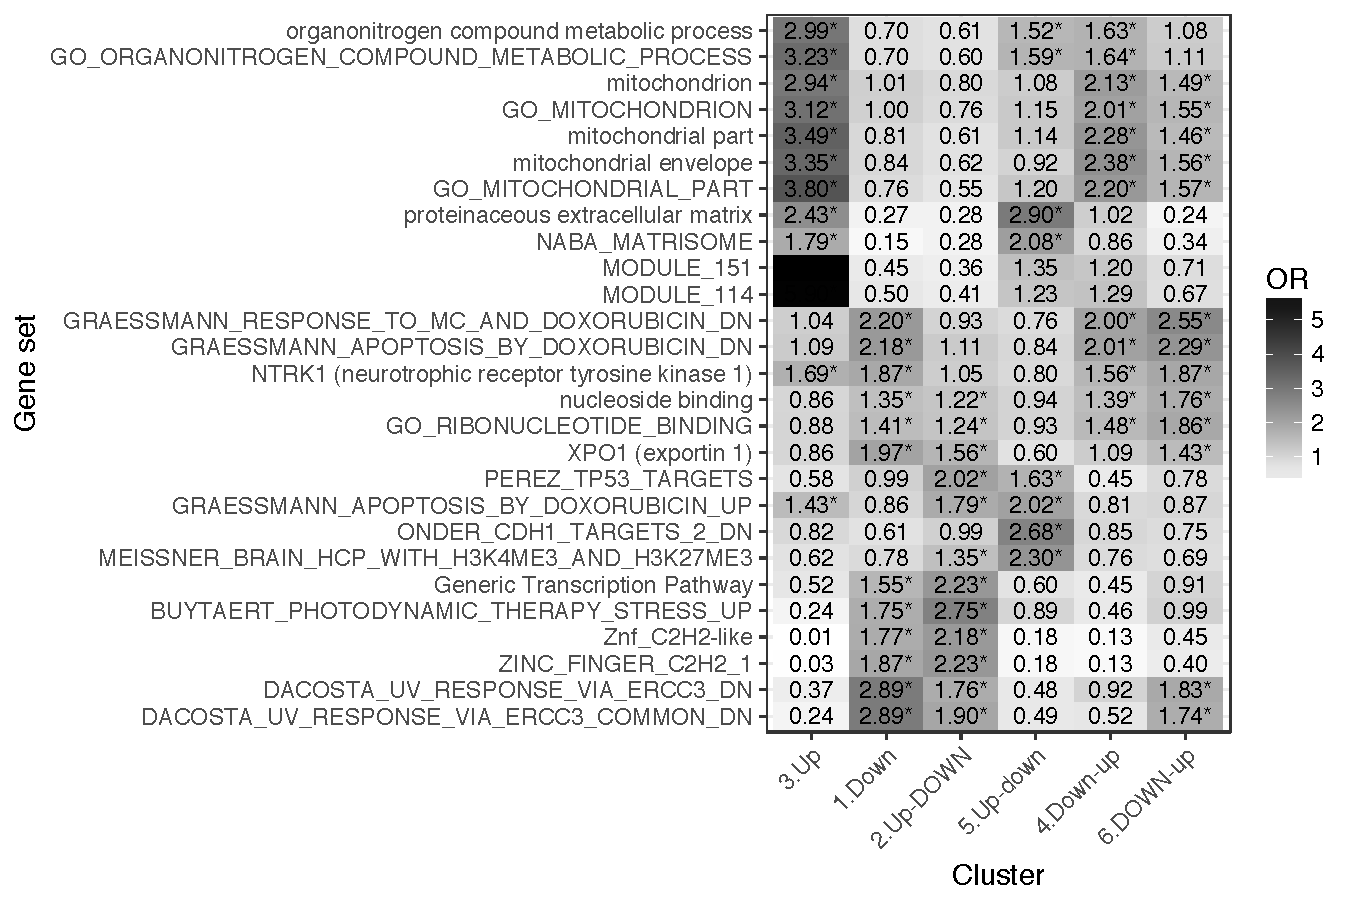
\includegraphics[width=1\textwidth]{../figures/cluster_go.pdf} % use small or
    \caption{\it{Gene set enrichment analysis of genes in each response cluster confirms expected patterns: metabolic, mitochrondrial and DNA damage processes, as well as existing doxorubicin response genes.}}
    \label{fig:go}
    \end{center}
\end{figure}

\begin{figure}[h]
\begin{center}
    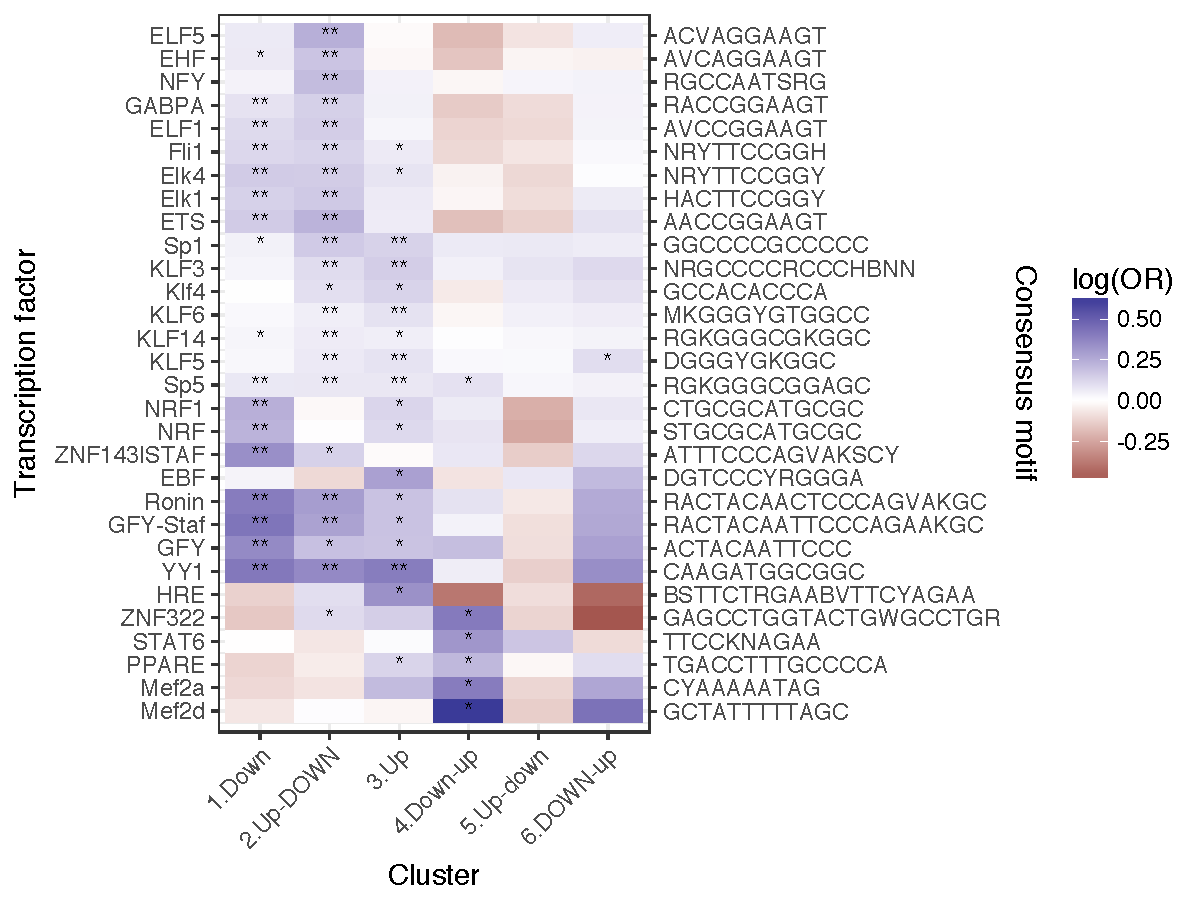
\includegraphics[width=1\textwidth]{../figures/cluster_tf.pdf} % use small or
    \caption{\it{Enrichment of transcription factor binding motifs for each response pattern, using HOMER. ** denotes $q<0.05$, * denotes $q<0.5$.}}
    \label{fig:tf}
    \end{center}
\end{figure}

\begin{figure}[h]
\begin{center}
    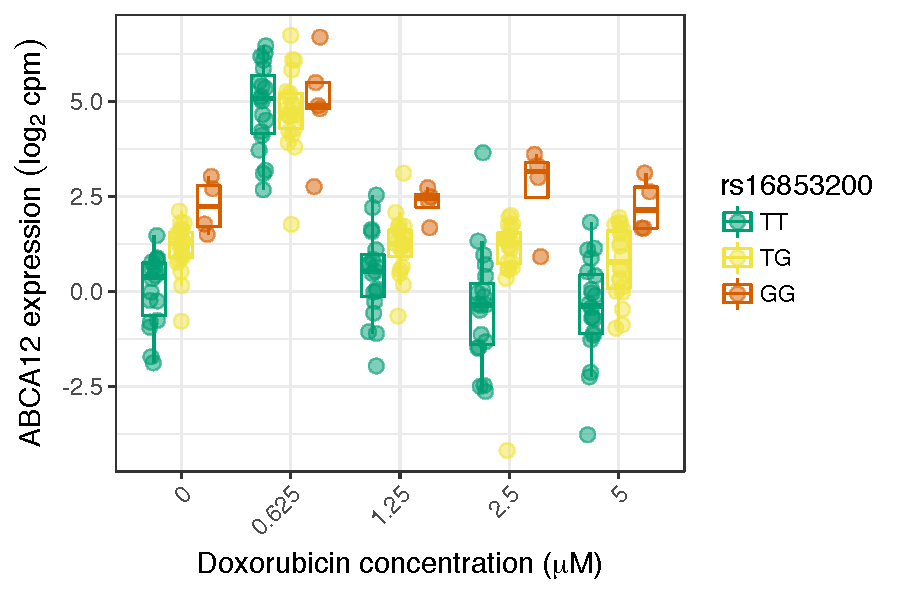
\includegraphics[width=.6\textwidth]{../figures/ABCA12.pdf} % use small or
    \caption{\it{An example response expression QTL that may act through buffering at high expression levels.}}
    \label{fig:ABCA12}
    \end{center}
\end{figure}

\begin{figure}[h]
\begin{center}
    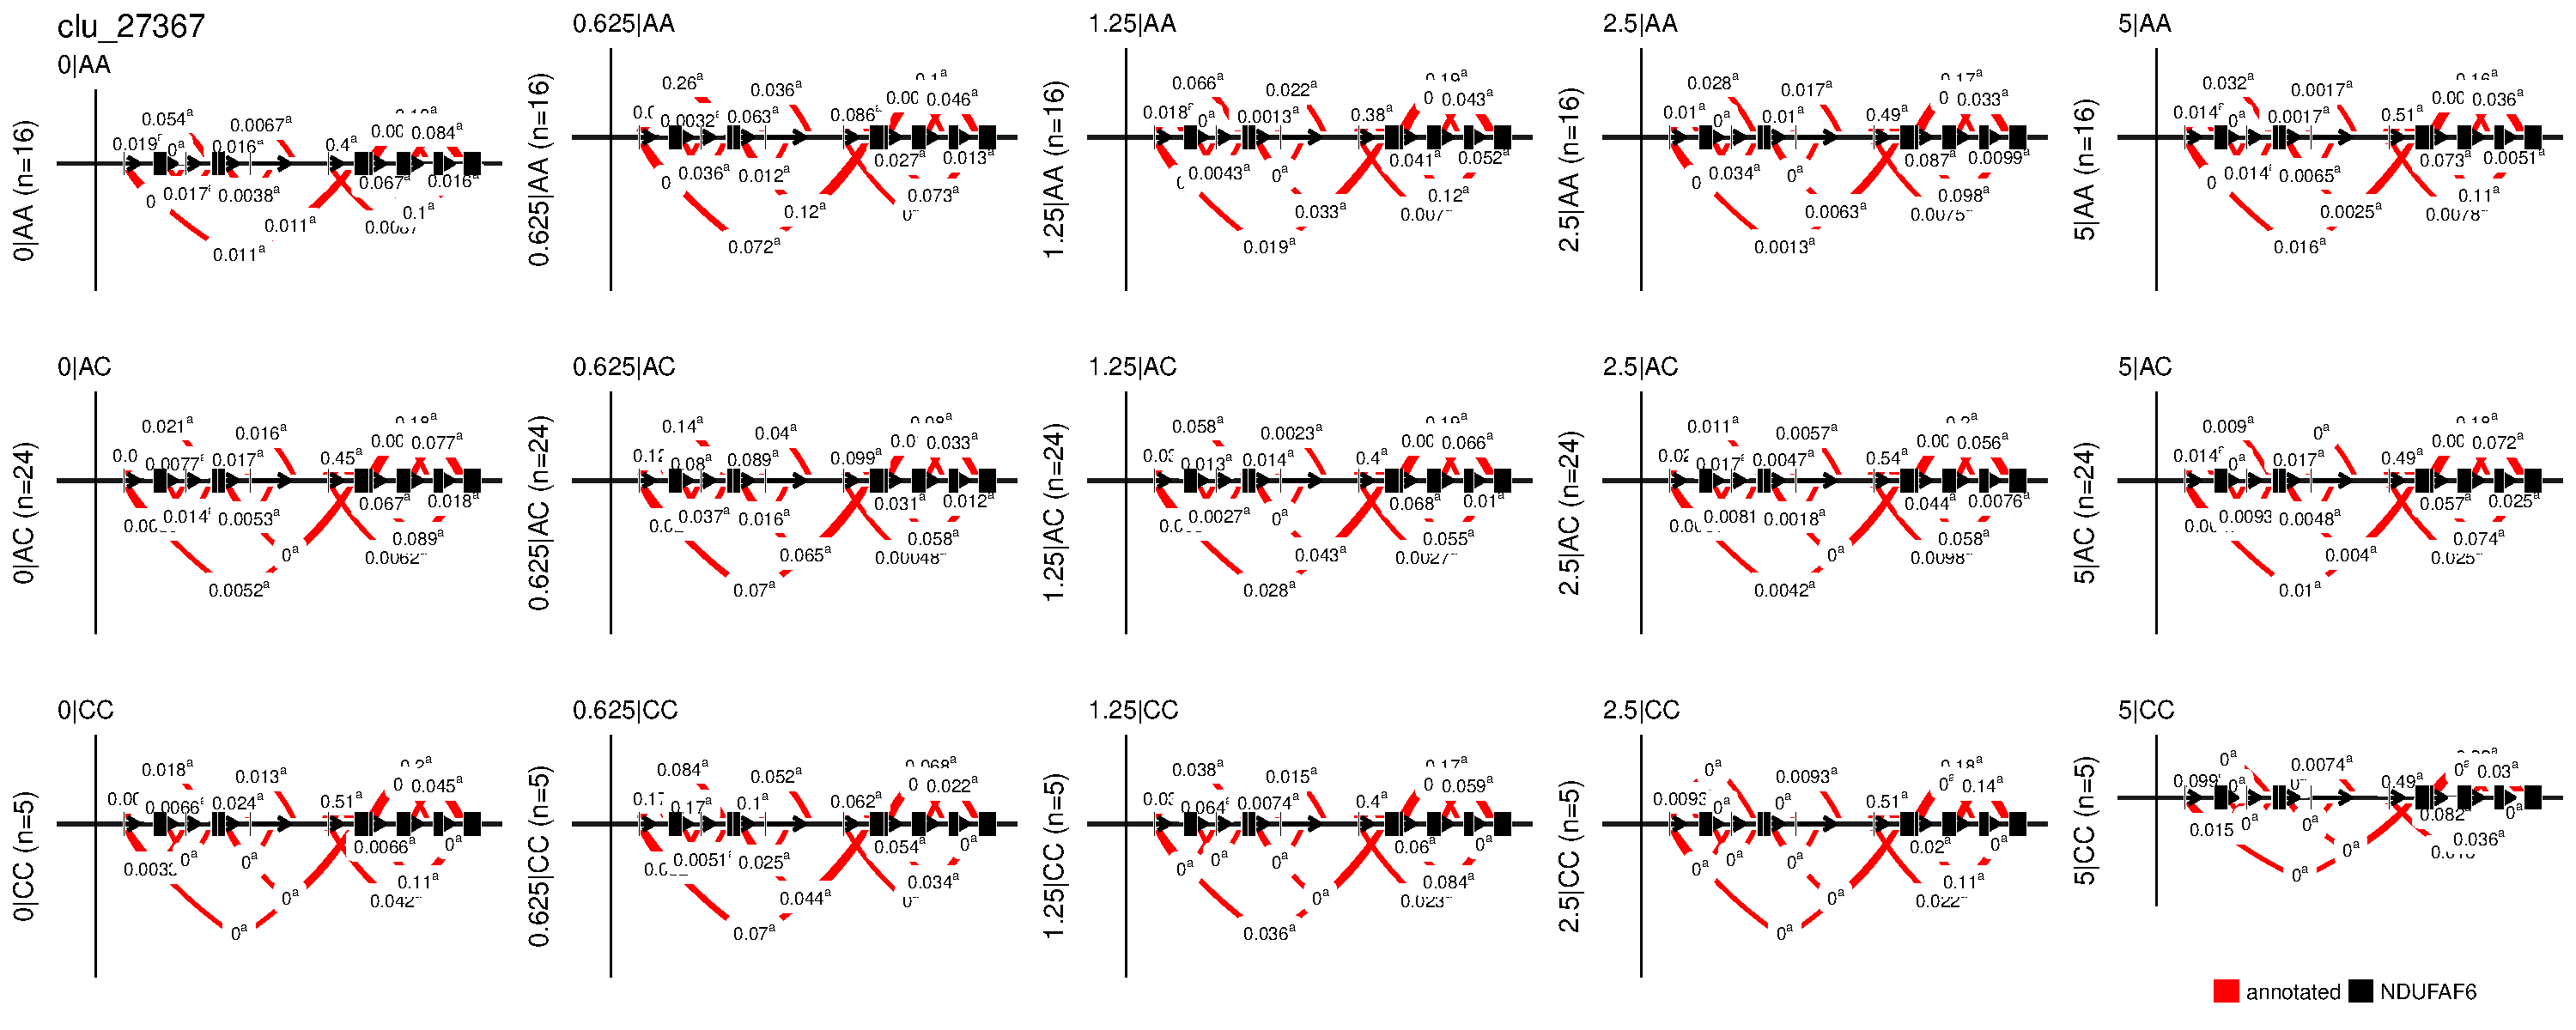
\includegraphics[width=1\textwidth]{../figures/rsQTL/NDUFAF6.pdf} % use small or
    \caption{\it{Doxorubicin exposure results in the use of a downstream alternative TSS which uncovers an association between rs896853 genotype and inclusion of the exon at chr8:94975318-94975415.}}
    \label{fig:NDUFAF6}
    \end{center}
\end{figure}

\bibliography{dox}     
\end{document}